\chapter{GPU Computing}

\section{OpenGL}
* basic introduction of OpenGL as standard cross-platform graphics library


* talk about gpu hardware in relation to graphics, segway into GPGPU


\section{General Purpose GPU Programming}

* give motivations for GPGPU, brief history


* overview of GPU memory hierarchy


* what kind of algorithms are good fit, performance primitives

\section{OpenCL}

* design goals
    open standard
    heterogeneous environment

* concept of kernels 


* talk about contexts and command queues briefly


* compare with CUDA briefly


\subsection{memory}
* Brief overview of the different types of memory and their speeds
\begin{figure}[!htc]
 		\centering
		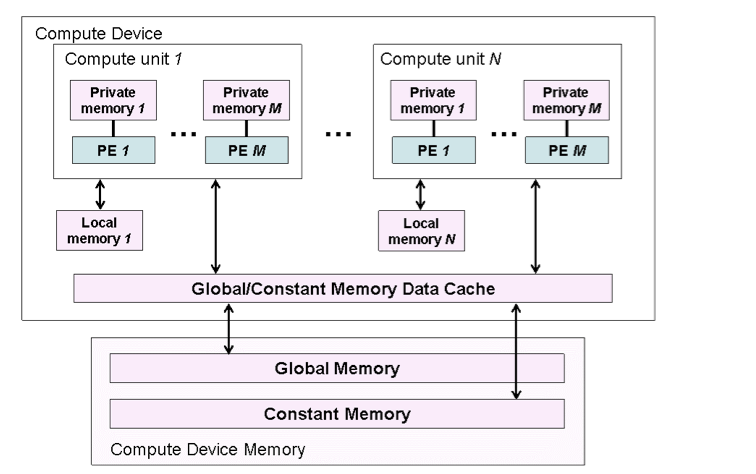
\includegraphics[scale=0.5]{figures/gpu_memory.png}
		\label{fig:logic}
        \caption{ Standard Memory Heirarchy Diagram }
\end{figure}

We pass data to the gpu and try to keep it there, no cost between kernels


\subsection{float4}
The OpenCL 1.0 specification defines the \verb|float4| type as a vector of four
floating point numbers. Since our simulation is designed to be 3 dimensional it
is the most convenient data type for storing arrays of coordinates. The OpenCL
1.1 standard does define a \verb|float3| type, but as of this writing the 1.0
standard is still the most widely available implementation so we use \verb|float4|
for backwards compatibility. We have also found it convenient to package many
variables into a single array for use on the GPU, and we are able to utilize
the unused components of 3 dimensional vectors for storing some scalar values.

\subsection{C++ Wrappers}
* discuss wrappers provided by Khronos


* our wrappers


\subsection{CL/GL Interoperability}
* sharing memory context to avoid transfer over PCI bus


* issue on the mac, had to edit the header

\subsection{Timing}
* gpu timers


